\subsection{Genome Instrumentation}
\label{sec:genome-instrumentation}

This section reviews hereditary stratigraphy as originally developed for inference over asexual populations then introduces gene- and species-level hereditary stratigraphy instrumentation strategies designed for sexual populations.
Subsequent discussion covers recombination and ``gene drive'' mechanisms employed for species-level instrumentation.


% \begin{figure}
  \centering
  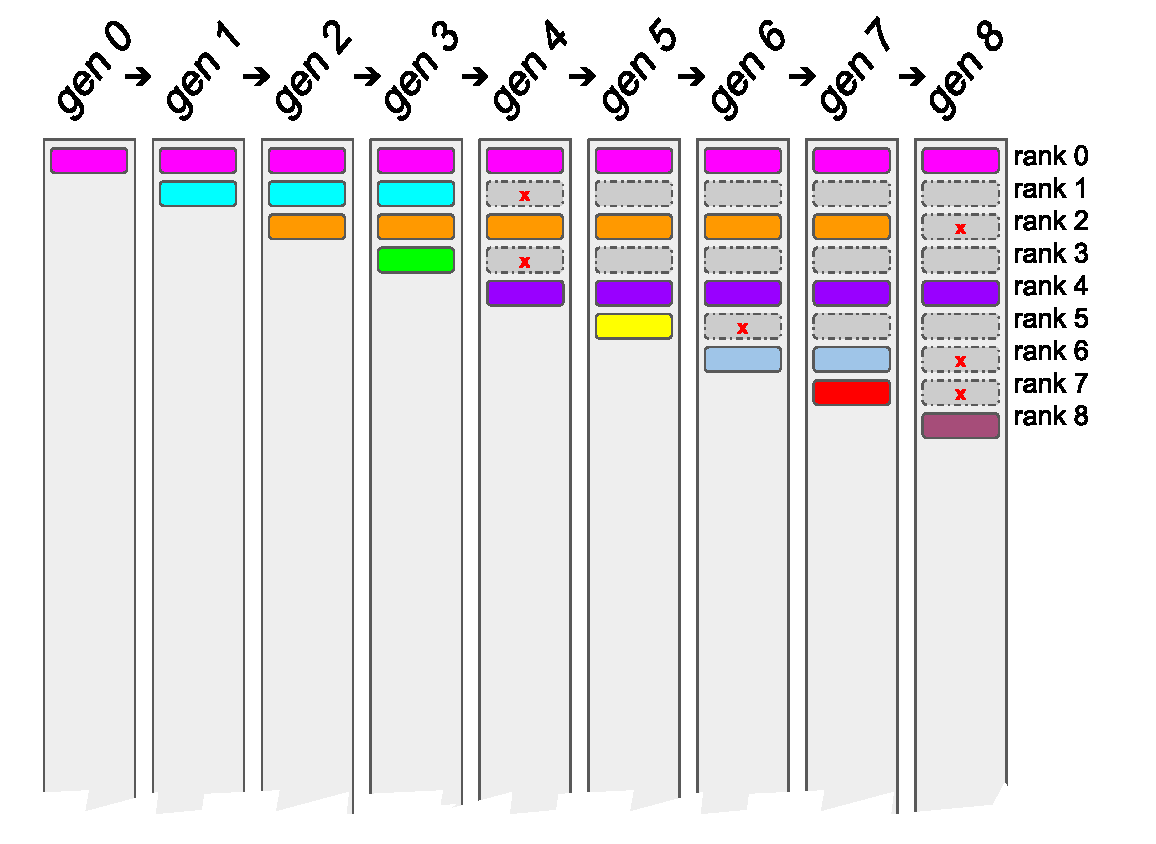
\includegraphics[width=\textwidth]{img/deposit-prune-example}
  \caption{
    TODO
  }
  \label{fig:deposit-prune-example}
\end{figure}

% \begin{figure}
  \centering
  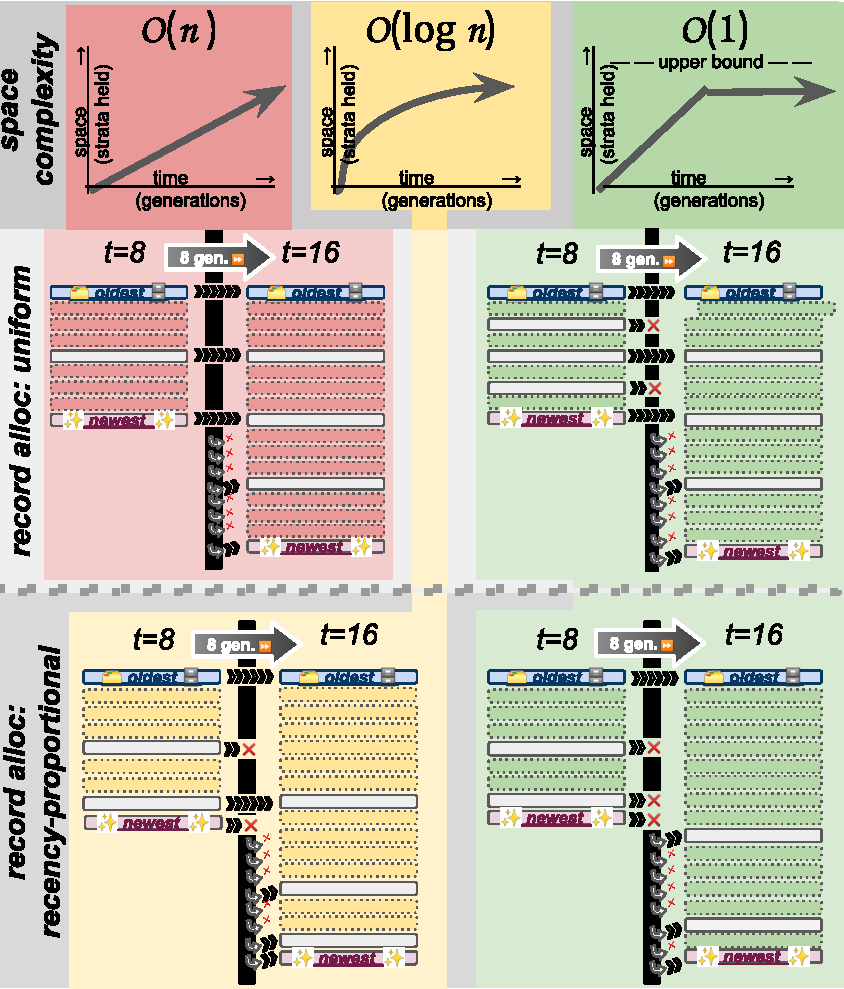
\includegraphics[width=\textwidth]{img/retention-policy-matrix}
  \caption{
    Comparison of four stratum retention policies by space complexity per stratigraph with respect to generations elapsed (columns, red/yellow/green) and by distribution of retained differentia (rows).
    Uniform allocation keeps differentia in evenly-spaced layers.
    Recency-proportional allocation keeps more more-recent differentia, trading off coarser resolution to infer ancient phylogenetic events for finer resolution to infer recent phylogenetic events.
    Retained layers under each policy are shown at $t=8$ generations and $t=16$ generations, with new differentia being deposited in a descending fashion.
    Differentia pruning events are noted with a red $x$.
  }
  \label{fig:retention-policy-matrix}
\end{figure}

\textbf{Hereditary Stratigraphy.}
Proposed methods for genealogical and evolutionary inference over distributed sexual populations draw on ``hereditary stratigraphy,'' originally developed to facilitate phylogenetic inference over asexual populations \citep{moreno2022hstrat}.
The core mechanism of this technique is generation-on-generation accumulation of randomized ``fingerprint'' packets.
Offspring inherit parents' fingerprints and append a new entry.
This process repeats with the next generation.

Each accumulated fingerprint ultimately serves as a kind of linealogical checkpoint.
Because fingerprints are faithfully inherited each generation after their creation, discrepancy between coincident fingerprints held by two population members implies divergent ancestry at their shared time point.
So, last common ancestry necessarily precedes the first mismatching fingerprints.
Fingerprint values convey no function phenotypic information.
Rather, they should be considered simply as neutral ornamentation affixed to an underlying functional genome to instrument it.
Because they tag along with genomes across replication events, a system's phylogenetic history can be reconstructed by proxy based on these instruments.

Some attention must be paid to memory footprint.
Proceeding naively, fingerprint accumulation with each generation would hopelessly bloat annotation size.
Fortunately, the underlying inferential mechanism supports thinning out of fingerprints.
Pruned-away fingerprints introduce uncertainty into estimation of two records' divergence generation.
If every other fingerprint was pruned, for example, divergence generations would only be estimable to within 2 generations.
In this way, configuration of what fingerprints to keep when directly administers underlying trade-offs between memory use and inferential power.
Although beyond present scope, significantly more can be said about fingerprint curation.
For detail, refer to \citep{moreno2022hereditary}.

To simplify experimental setup and analysis, experiments reported here do not incorporate fingerprint pruning.
However, all inference mechanisms introduced here are, in principle, compatible with fingerprint pruning.
Further work remains to directly investigate how pruning affects presented approaches' characterization of evolutionary history and dynamics.
Analogous work in asexual populations should provide some initial indications in this direction \citep{moreno2023toward}.

This work uses 64 bit fingerprints, which collide spuriously with negligible probability $2^{-64} \approx 5 \times 10^{-20}$.
At population size 100 over 200 generations, as in the first sets of reported experiments, the probability of any collision is miniscule: $< 2 \times 10^{-15}$.
At population size 200 over 400 generations, as in the last set of reported experiments, the probability of any collision is also miniscule: $< 5 \times 10^{-15}$.

\begin{SCfigure}[3][b]
  \centering
  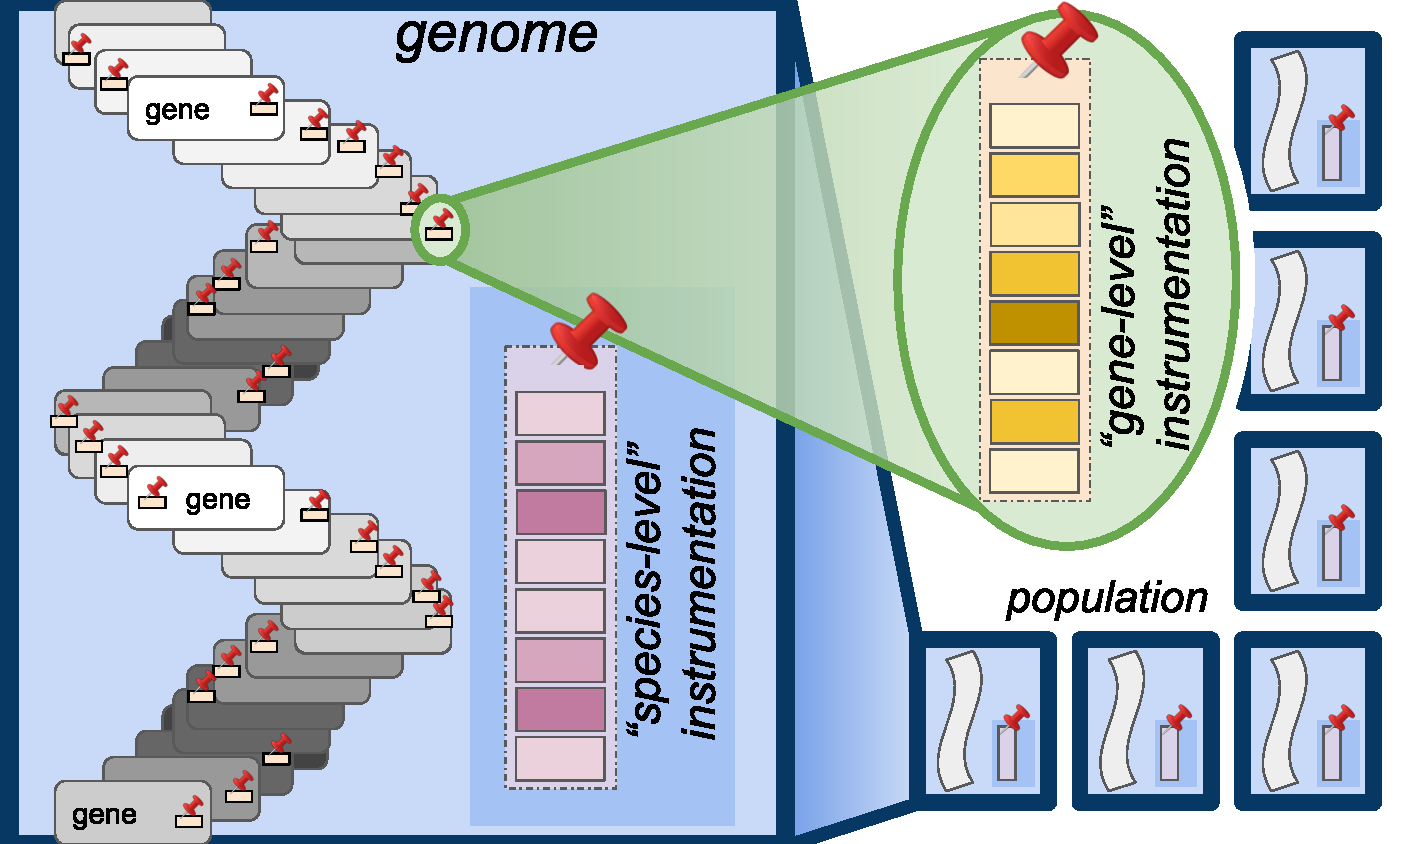
\includegraphics[width=0.5\textwidth]{img/annotation-types}
  \caption{
    Proposed instrumentation methods: ``species-level'' and ``gene-level'' instrumentation.
    Each organism has a single hereditary stratigraph attached as species-level instrumentation, with a gene drive mechanism (Figure \ref{fig:gene-drive}) ensuring consistentcy within species (i.e., interbreeding populations).
    Gene-level instrumentation associates instrumentation with individual genes, to be used for gene tree reconstructions.
  }
  \label{fig:annotation-types}
\end{SCfigure}

\textbf{Sexual Instrumentation Schemes.}
As originally devised for asexual populations, hereditary stratigraph annotations assign one-to-one with genomes.
Here, we explore two alternate schemes designed for instrumentation of sexual populations: ``gene-level'' and ``species-level'' instrumentation.
Figure \ref{fig:annotation-types} compares these two schemes.

Gene-level instrumentation views individual genes simply as asexual atoms, and instruments them individually.
Reconstructions, therefore, operate along the lines of ``gene tree'' analsyes in traditional phylogenetics \citep{avise1989gene}.
In some cases, it may make sense to instrument every gene independently.
Other applications may warrant instrumenting only a subset of genes or introducing instrumented ``dummy'' genes.

Species-level instrumentation associates one instrument per genome but these instruments adopt a consensus value within species populations.
Consensus arises through a ``gene drive'' mechanism (described below) that forces a single fingerprint value to sweep each fingerprint layer within an interbreeding subpopulations.

Species-level instrumentation powers genealogical inference (Section \ref{sec:genealogical-inference}) and population size inference (Section \ref{sec:population-size-inference}).
Gene hereditary stratigraph instrumentation powers positive selection inference (Section \ref{sec:selection-inference}).

\begin{SCfigure}[3][b]
  \centering
  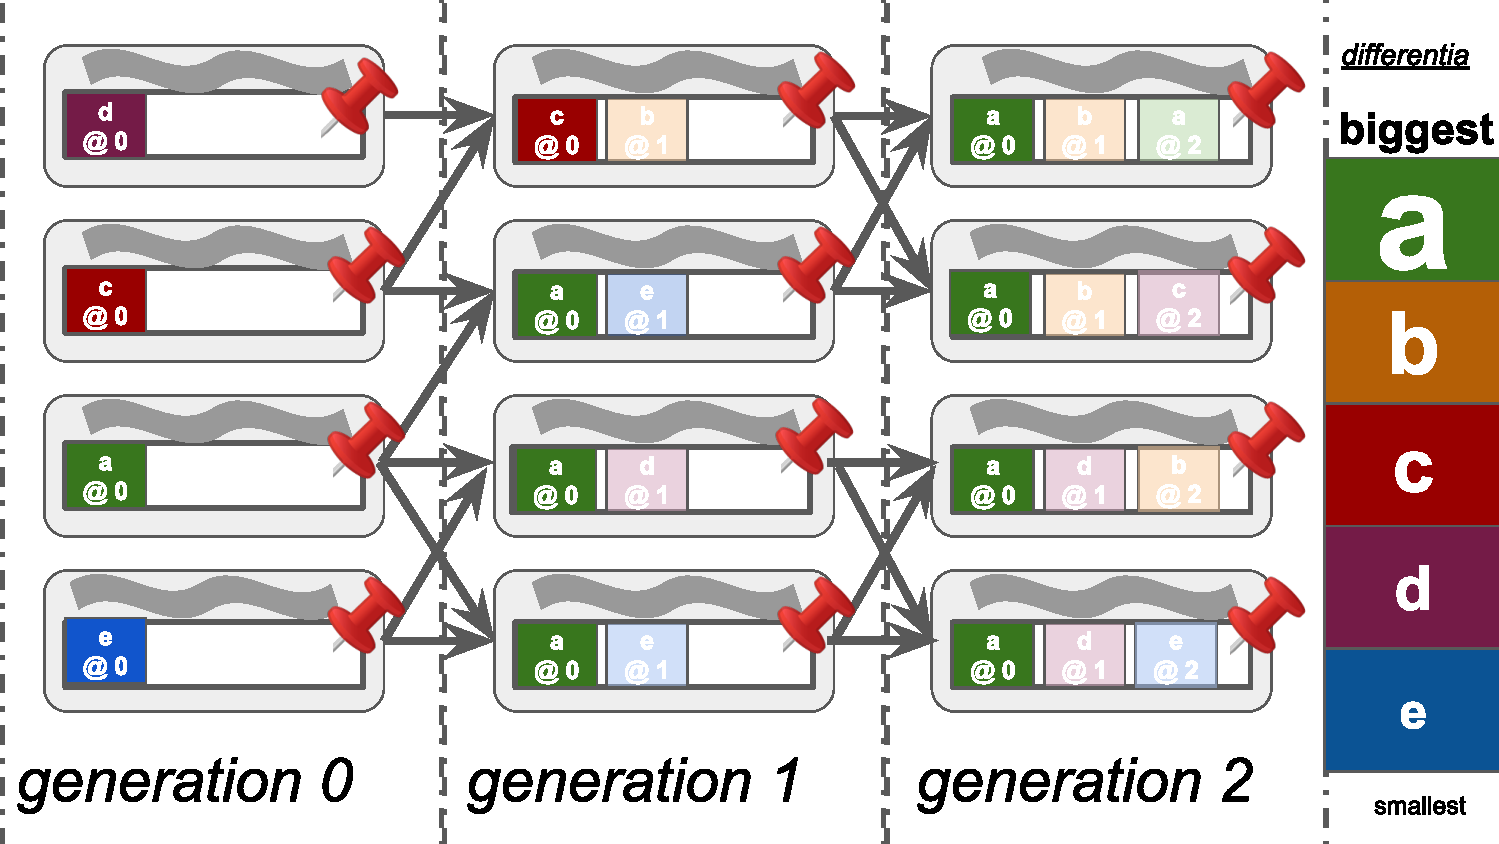
\includegraphics[width=0.6\textwidth]{img/gene-drive}
  \caption{
    Gene drive mechanism for species-level instrumentation.
    The larger of parents' differentia values at each layer is inherited.
    The largest value generated among layer 0 differentia ($a$) spreads from one member at generation 0 to all four by generation 2.
    This mechanism applies to ``species-level'' instrumentation (Figure \ref{fig:annotation-types}).
  }
  \label{fig:gene-drive}
\end{SCfigure}

\textbf{``Gene-drive'' Recombination Mechanism.}
Species-level tracking relies on consensus among fingerprint values within reproductively isolated subpopulations.
Drift will ultimately yield consensus, but expected coalescence times can be long for large populations
A simple inheritance rule reaches consensus faster: inherit the larger of parents' fingerpint values.
Global maximum fingerprint values will spread rapidly and fix.
Figure \ref{fig:gene-drive} depicts this mechanism.

Asynchronous generations slightly complicate the picture.
When individuals from different generations recombine, one parent will have fingerprint layers absent in the other.
How should recombination proceed in this case?
One possibility would be to simply ``fast forward'' the younger instrument to match the generational depth of the elder.
However, like with fingerprint pruning above, full consideration remains for future work.
All reported experiments use synchronous generations.

The gene-drive-based recombination mechanism described in this section applied exclusively to species-level instrumentation.
(Gene-level instruments, although tagging along with genes shuffled up through genome-level recombination, did not themselves recombine.)

\textbf{Fingerprint Collision Probability.}
Under gene-drive recombination, fixed fingerprints skew large due to the gene drive criterion.
This skew increases the probability of fingerprint collision between two populations which would cause spurious detection of shared ancestry.
We will assess the extent of this issue by computing threshold population sizes where collision probability becomes substantive.

Suppose independent populations of size $a$ and $b$.
The largest fingerprint in each population will drive to fixation.
If each population members' gene is drawn from uniform distribution on integers $[0, u)$, then the probability of collision between the populations' fixed genes can be derived as

\begin{scriptsize}
\begin{align*}
\frac{a}{a + b}\sum_{n=1}^{a + b - 1} \frac{u^{- n - 1} \left(\frac{u - 1}{u}\right)^{a + b - n - 1} \left(1 - \frac{{\binom{a - 1}{n}}}{{\binom{a + b - 1}{n}}} \right) {\binom{a + b}{n + 1}}}{1 - \left(\frac{u - 1}{u}\right)^{a + b - 1}}
+ \frac{b}{a + b} \sum_{n=1}^{a + b - 1} \frac{u^{- n - 1} \left(\frac{u - 1}{u}\right)^{a + b - n - 1} \left(1 - \frac{{\binom{b - 1}{n}}}{{\binom{a + b - 1}{n}}} \right) {\binom{a + b}{n + 1}}}{1 - \left(\frac{u - 1}{u}\right)^{a + b - 1}}.
\end{align*}
\end{scriptsize}
% Derivation will be provided in supplementary materials. TODO?

For 32-bit differentia $u = 2^{32}$, collision occurs with $p < 0.5$ ($p = 0.46$) for populations of size $a = b = 2^{32}$.
Collision occurs with $p < 0.01$ for populations of size $a = b = 2^{26}$.
So, 32-bit fingerprints can differentiate species pairs of around $6.7 \times 10^{7}$ members each with reasonable consistency.%
\footnote{
Reported experiments used 64-bit fingerprint values, which will exhibit even lower collision probabilities.
However, numerical considerations impede precise calculation.
}
